\chapter{Results}

\emph{\color{gray}Was there something more you wanted to put in experimental?}

Studies of several emission peaks of neutral Ba in SXe are discussed in \ref{sec:fluorescence}.  Temperature and annealing dependence are discussed in \ref{subsec:tempanneal}.  Bleaching of these peaks is discussed in detail in \ref{subsec:bleaching}.  Imaging of Ba fluorescence in a focused laser region is discussed in \ref{imaging}, with the ultimate achievement of imaging at the single atom level using the 619-nm fluorescence peak.  Candidate fluorescence peaks of Ba\textsuperscript{+} in SXe are reported in \ref{sec:BaPlus}.

\section{Fluorescence of Ba in SXe}
\label{sec:fluorescence}

Deposits of Ba in SXe absorb primarily between 540~nm and 570~nm.  An absorption spectrum, obtained by observing absorption of white light by a large Ba deposit at 11~K, is shown in Fig. \ref{fig:BaAbs}, along with an example emission spectrum.  Significant broadening, as well as a 4-nm redshift  of the central peak, occur relative to the vacuum $6s^{2}$ $^{1}$S$_{0} \rightarrow 6s6p$ $^{1}$P$_{1}$ absorption value of 553.5~nm.  The observation of the same absorption and emission spectra with deposits made with the Ba\textsuperscript{+} ion beam as with the neutral Ba getter source demonstrate some neutralization of the ions.  The fraction of ions neutralized is not determined.  \cite{Mong2015,Shon,Brian}

\begin{figure} %[H]
        \centering
                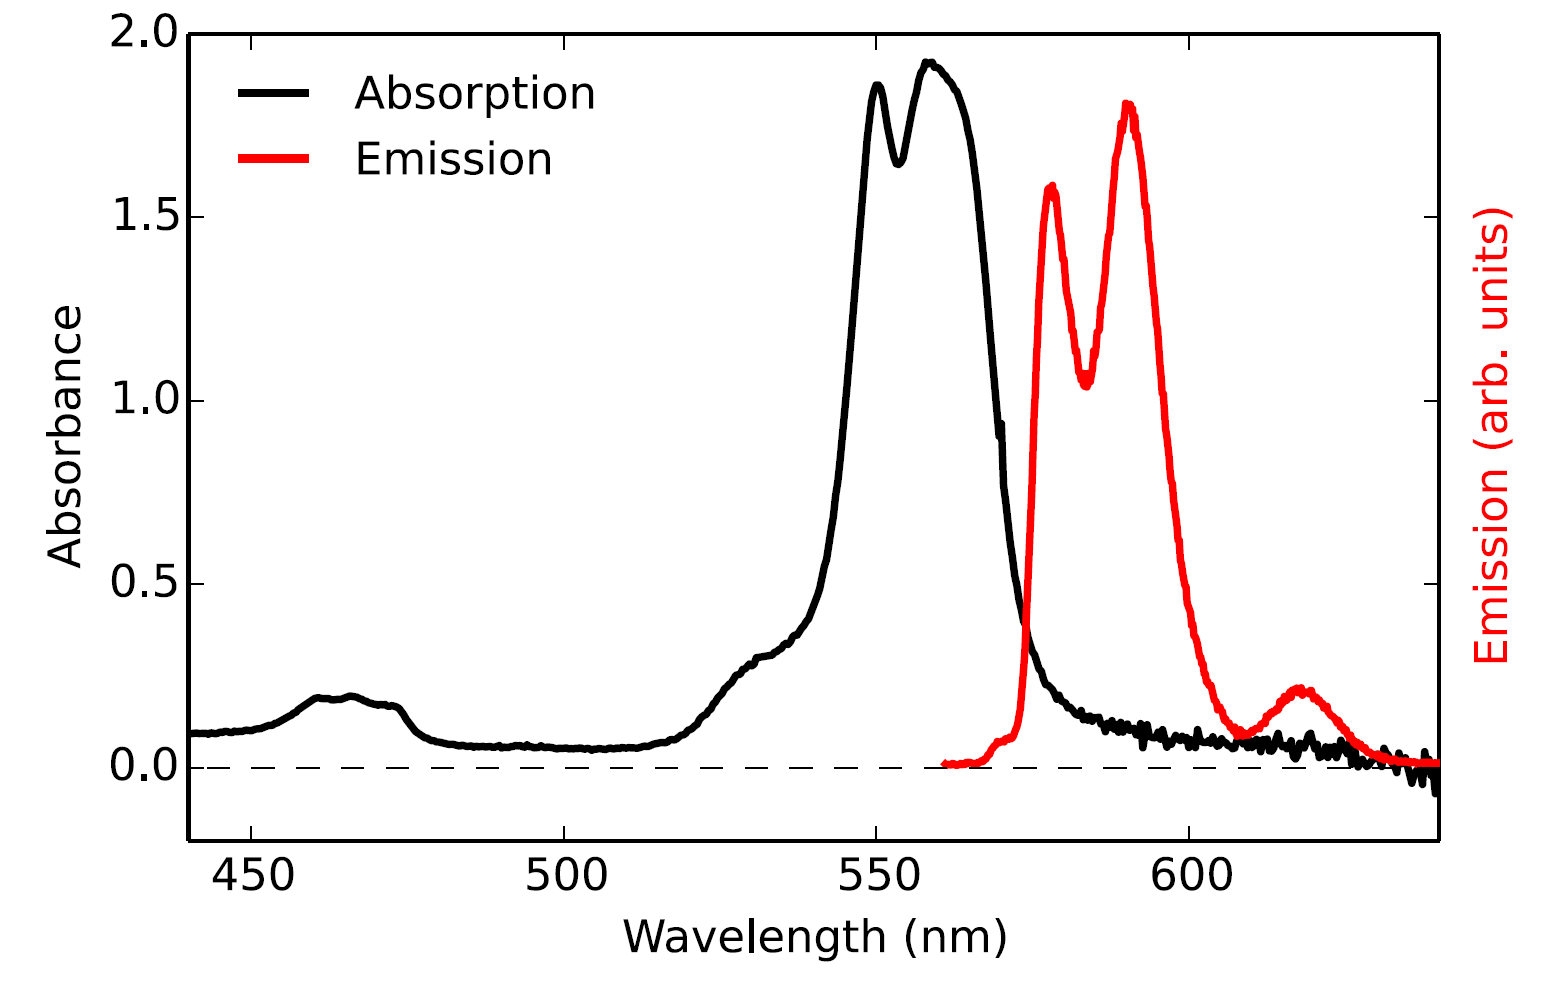
\includegraphics[width=.7\textwidth]{figures/BaAbs_fromBaSpec.png}
                \caption{\color{red}Get rid of the (a).  Probably need to just edit screenshot with paint.  \cite{Mong2015}}
\label{fig:BaAbs}
\end{figure}

The several red-shifted emission peaks observed are attributed to Ba atoms occupying different matrix sites in the SXe.  Deposition at temperatures higher than 11~K and exploration of more excitation wavelengths have led to discovery of a few emission peaks beyond the 591- and 577-nm peaks reported in \cite{Shon} and \cite{Brian}.  Emission spectra for selected excitation wavelengths are shown in Fig. [excit a], for a deposit made at 44~K and observed at 11~K.  These selections are part of a full excitation spectrum, shown in Fig. [excit b].

\begin{figure} %[H]
        \centering
                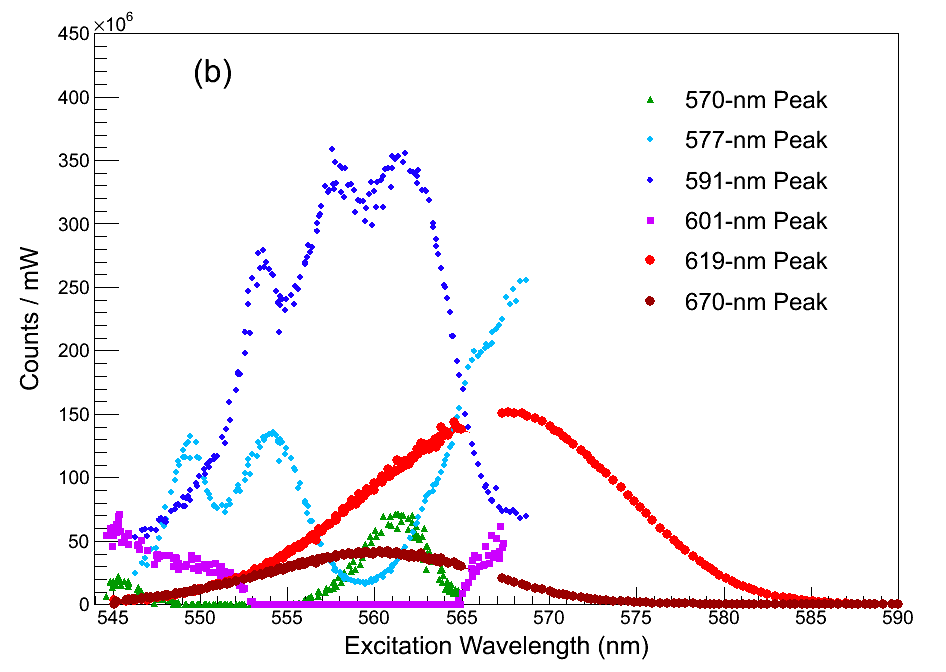
\includegraphics[width=.7\textwidth]{figures/excitspec_grn.png}
                \caption{{\color{red}Fluorescence spectra for a few different excitation wavelengths (a)} and full excitation spectra (b) for all observed Ba fluorescence peaks.  Magnitudes have been scaled for visibility on the same plot (relative magnitudes are arbitrary as they are affected by relative site populations and fluorescence efficiencies).  The discontinuity around 566~nm for the 619- and 670-nm peaks is the boundary between usage of different laser dyes.  R6G dye is used for higher wavelengths and R110 for lower wavelengths and for all other curves.  Curves for the R6G segments (619- and 670-nm peaks) require special scaling to line up with their respective R110 segments, and this scaling was different between the 619- and 670-nm peaks, likely due to different relative populations of those sites on the different deposits.}
\label{fig:excitspecGrn}
\end{figure}

\subsection{Annealing/Temperature Dependence}
\label{subsec:tempanneal}

\emph{\color{gray}When does it need to be mentioned that certain data was also used in the paper(s)?}

Matrix site occupancies for Ba atoms can depend on annealing history, and similarly on the temperature at which a deposit is made.  \emph{\color{gray}Annealing plots -- all peaks or just the ones shown in the paper? ... and point out that the plots also show the lower fluorescence at higher temp, which though comes back when returning, i.e. efficiency is lower at higher temp, which has implication for nEXO probe and Adam.  Probably show the spectrum plot like in Ba Spec too.}

Depositing at around 50~K also results in higher signal, vs. depositing at the observation temperature of 11~K, as shown in Fig. [fig of higher 619? other peaks?].

\emph{\color{gray}Care about 10~K excitation spectrum?}

\subsection{Bleaching}
\label{subsec:bleaching}

({\color{red}do a correction on p-meter sensitive area and on p-meter quantum efficiency, and also a spherical aberation correction for power, though that may not matter for the defocused studies.})

590 etc, model fit (see results intro paragraph)

\begin{figure} %[H]
        \centering
                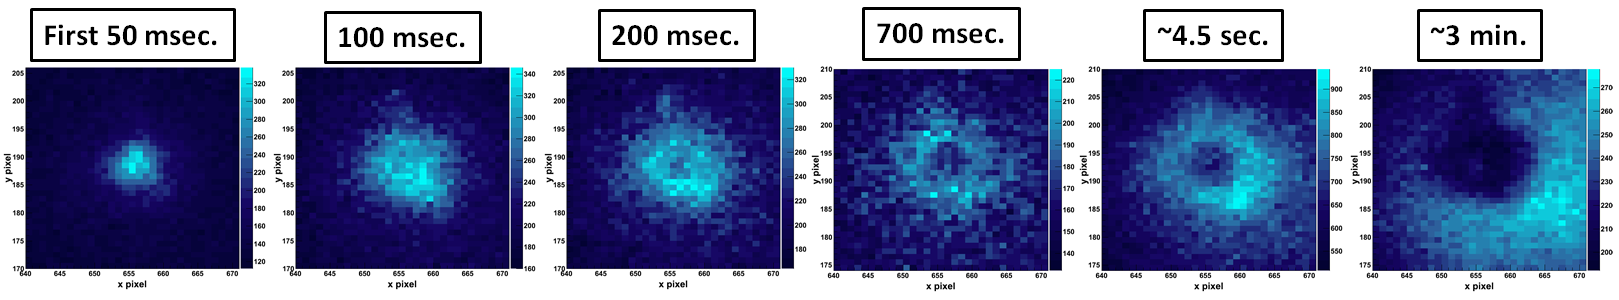
\includegraphics[width=.9\textwidth]{figures/hole_bleach_590.png}
                \caption{}
\label{fig:testfig}
\end{figure}

619, with the changes in time and I

bleaching effect on excit spec (bleaching site change search)

\section{Backgrounds}
\label{sec:bgs}

Show Cr$^{+++}$ excit spec agreement with old paper for calling broad stuff also due to that.

\section{Imaging}
\label{imaging}

\subsection{Imaging 577- and 591-nm peaks}

\subsection{Imaging 619-nm peak}

\begin{figure} %[H]
        \centering
                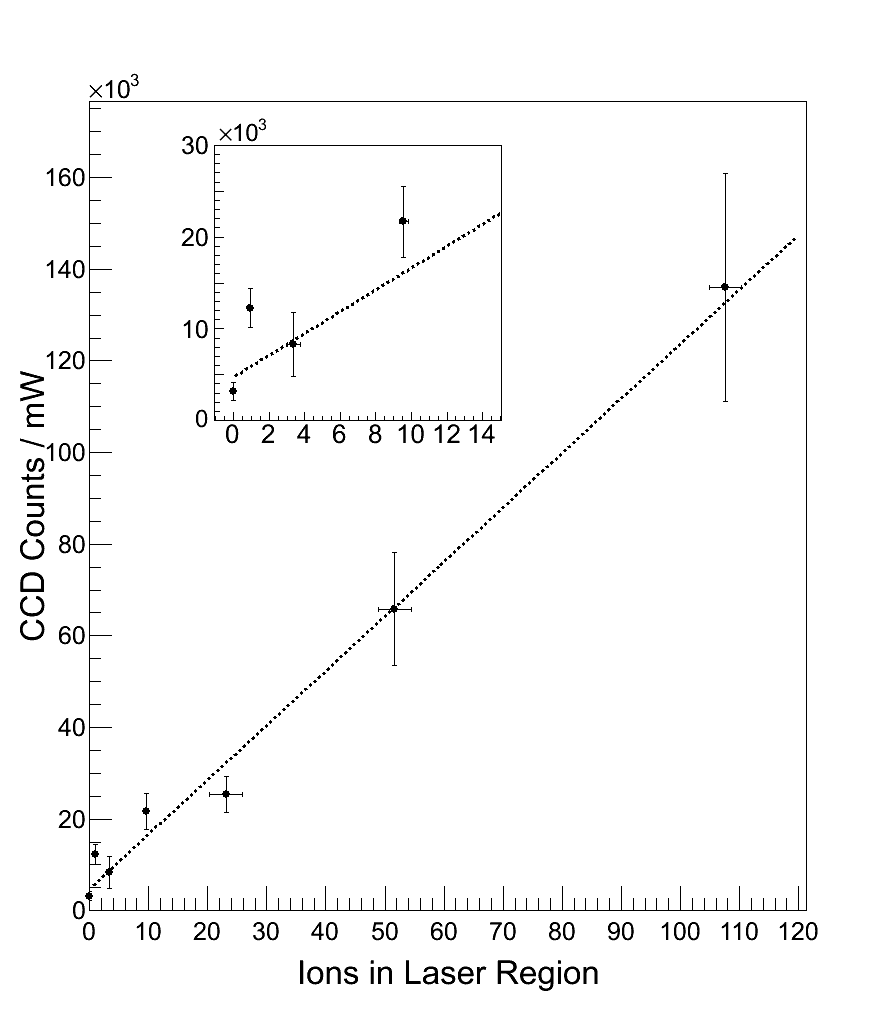
\includegraphics[width=.7\textwidth]{figures/fitgrouped_20150807_20150916_inset.png}
                \caption{Combined 2015-08-07 and 2015-09-16 with statistical errors.  \emph{\color{gray}Move y-axis title over.}}
\label{fig:lin}
\end{figure}

\subsection{Further Checks on 619-nm Peak}

\emph{\color{gray}getter and Ar$^{+}$ for 619 \textbf{\color{gray}This section was claimed in Ba getter section of Chapter 3 to talk about getter use in identifying 619.}}

Also have stuff on ruling out extra-BP stuff, and something else I think.

Leak rate dependence -- ``Leak rates resulting in [x nm/s $\rightarrow$ 1:xxx Ba:Xe] optimize fluorescence, which is consistent with rates where Ba-Ba interactions are minimized [ref?] \emph{\color{gray}(are there other explanation?  check the gas oxidation thing.)}.  Rates higher than this result in rapid frosting ..." \emph{\textbf{\color{gray}May also just put this at the end of the  Fluorescence section.}}

\section{Candidate Ba\textsuperscript{+} Lines}
\label{sec:BaPlus}